\documentclass[12pt,french]{article}

\usepackage[utf8]{inputenc}
\usepackage[T1]{fontenc}

\usepackage{hyperref}
\usepackage{graphicx}
\usepackage{float}
\usepackage{babel}
\usepackage{longtable}
\usepackage{tabularx}
\usepackage{enumitem}

\title{SMOC - Rapport du Projet BUMPERS}
\author{Corentin Dupret, Sami Tabet}
\date{\today}

\begin{document}

\maketitle

\newpage

\tableofcontents

\newpage

\section{Introduction}

Le jeu BUMPERS est un jeu où il y a un arbitre et des joueurs. Chaque joueur gère le mouvement d'une bille à l'aide de l'accéléromètre d'un microcontrôleur. L'arbitre place chaque bille sur le plateau dans l'ordre d'arrivée des joueurs. Puis, l'arbitre lance le jeu et gère le mouvement des billes à partir des informations envoyées par les joueurs. Ceux-ci doivent diriger leur bille vers les autres pour provoquer des chocs, comme au billard. Le but est de faire sortir les billes des autres joueurs du plateau car elles sont ainsi éliminées. Le dernier joueur dont la bille reste sur le plateau a gagné le jeu.

Le projet consiste en la création d'un client permettant de jouer au jeu BUMPERS avec d'autres clients. Le client est composé de deux microcontrôleurs STM32F4DISCOVERY, connectés entre eux, qui communiquent avec l'arbitre (c'est-à-dire le serveur) par fréquence radio.

\begin{figure}[h]
\centering
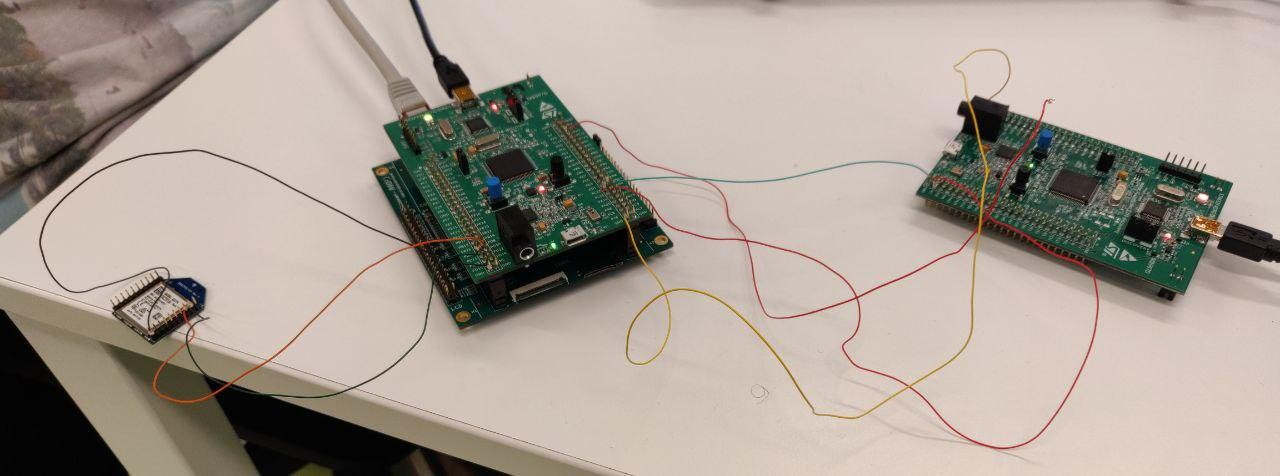
\includegraphics[width=\textwidth]{smoc_photo.jpg}
\caption{Photo du projet}
\label{fig:photo}
\end{figure}

\section{Architecture du projet}

\begin{figure}[H] 
\centering
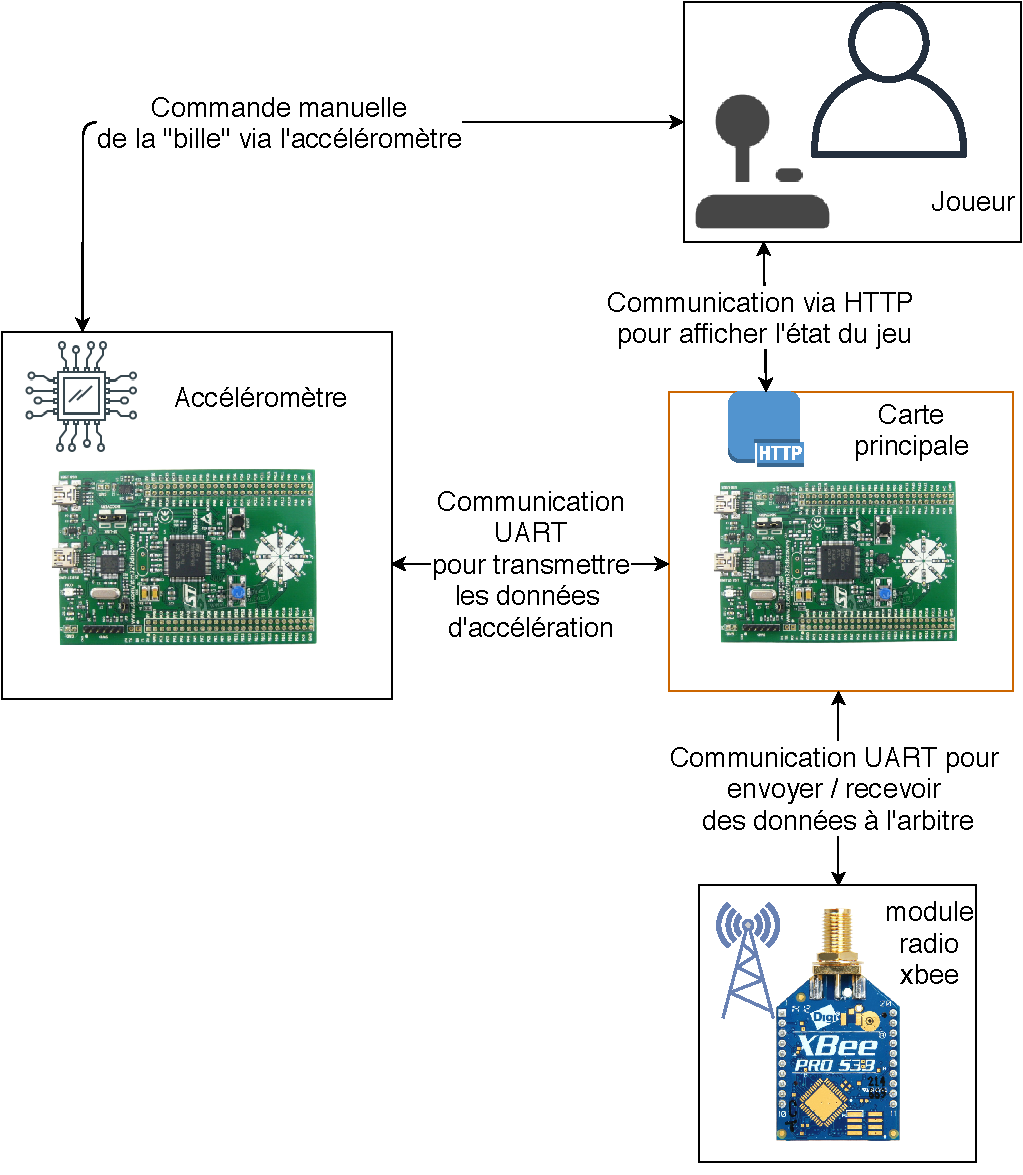
\includegraphics[width=\textwidth]{smoc_diagram.pdf}
\caption{Schéma de l'architecture du projet}
\label{fig:diagram}
\end{figure}

Le projet se découpe en plusieurs composants intéragissant entre eux pour former le client :

\begin{itemize}
    \item Un DevKit407 complet faisant tourner une interface web.
    \item Un module radio XBee permettant de communiquer avec l'arbitre par radio. Le joueur envoie les accélérations pour contrôler la bille tandis que l'arbitre envoie l'état du jeu avec, notamment, la position de la bille de chaque joueur.
    \item Une connexion UART entre le DevKit407 et le XBee.
    \item Un STM32F4DISCOVERY sans DevKit chargé de récupérer les données de l'accéléromètre MEMS intégré. Le joueur peut contrôler le mouvement de sa balle en bougeant ce microcontrôleur dans l'espace.
    \item Une connexion UART entre les deux microcontrôleurs pour permettre au STM32F4DISCOVERY de communiquer avec le DevKit407.
    \item Une connexion Ethernet entre le DevKit407 et un ordinateur pour permettre au joueur d'accéder à l'interface web afin de prendre ses décisions en connaissance de cause.
\end{itemize}

La raison pour laquelle deux microcontrôleurs sont utilisés est que l'accéléromètre ne fonctionne pas avec le DevKit407, qui est nécessaire pour disposer d'une connexion Ethernet avec le joueur. Par conséquent, deux microcontrôleurs sont utilisés et communiquent en UART pour que le microcontrôleur principal (le DevKit407) puisse disposer des données de l'accéléromètre à envoyer à l'arbitre via le module radio, tout en exposant une interface web permettant au joueur de jouer en connaissant l'état du jeu à chaque instant.

Par conséquent, notre code source contient deux dossiers distincts, permettant de construire deux binaires différents : un pour chaque microcontrôleur. \texttt{acc} contient le code source pour le STM32F4DISCOVERY utilisant l'accéléromètre, tandis que \texttt{web} contient le code source pour le DevKit407 exposant l'interface web.

Le contenu de ces dossiers sera expliqué dans les différentes parties du rapport, avec des extraits de code source.

\section{Éxécuter le projet}

Pour éxécuter le projet, il faut au préalable construire les fichiers binaires des deux cartes:

\begin{itemize}
    \item La première responsable du serveur web et de la communication radio avec l'arbitre
    \item La seconde responsable de la partie accéléromètre
\end{itemize}

Pour cela il faut (pour chaque carte branchée en USB):

\begin{itemize}
    \item Aller dans le répertoire \texttt{web}/\texttt{acc} 
    \item Lancer la commande \texttt{make} pour construire le fichier \texttt{.elf} qui ira sur la carte
    \item ouvrir 2 terminaux
    \item dans le premier, lancer la commande \texttt{st-util} (outil installable depuis ici: \href{https://github.com/texane/stlink}{st-util})
    \item dans le second, lancer une session \texttt{gdb} (\textbf{attention}, ce doit être une session gdb compatible avec l'architecture de la carte, par exemple \texttt{arm-none-eabi-gdb} ou \texttt{gdb-multiarch})
    \item dans cette session \texttt{gdb}, lancer les commandes: 
    \begin{itemize}
        \item \texttt{target extended-remote :4242}
        \item \texttt{load build/web.elf} ou \texttt{load build/acc.elf} suivant la carte actuelle
        \item Une fois le chargement terminé, lancer la commande: \texttt{continue}
    \end{itemize}
\end{itemize}

\section{Étapes suivies}

Nous détaillons ici les différentes étapes suivies pour réaliser le projet, en expliquant le code source associé à chacune d'entre elles. Les étapes sont les suivantes :

\begin{itemize}
    \item Réalisation de l'interface web, avec l'affichage du plateau.
    \item Gestion de l'accéléromètre : récupérer les accélérations calibrées et les convertir (normaliser) avant l'envoi au second microcontrôleur.
    \item Gestion de la communication entre les deux cartes : le STM32F4DISCOVERY envoie les accélérations normalisées au DevKit407 qui les reçoit et les décode avant de les envoyer à l'arbitre.
    \item Intégration de la carte XBee au DevKit407 pour communiquer avec l'arbitre.
\end{itemize}

\subsection{Interface web et affichage du plateau}

Le projet (la carte \texttt{web}) dispose d'une interface web qui permet notamment d'afficher le plateau de jeu (les positions de toutes les billes en jeu) mais également de:

\begin{itemize}
    \item Lire des logs de debugging provenant du code relatif à la communication radio
    \item Configurer le baudrate à utiliser pour la communication radio
    \item S'assurer que la fonctionnalité de serveur web fonctionne correctement à l'aide de routes HTTP permettant d'allumer et d'éteindre des LEDs (permet d'aider le débugging).
\end{itemize}

Pour accéder à cette interface web il faut se connecter en ethernet sur la carte \texttt{web} (en configurant son ordinateur en réseau local) et aller sur la route: \texttt{192.168.1.29} qui a été définie au sein de CubeMX.

Les fichiers statiques sont stockés en tant qu'array de bytes dans le fichier binaire final pour éviter d'avoir à configurer un filesystem sur la carte.

Leur insertion est facilitée par des outils tels que \href{https://github.com/gwilymk/bin2c}{bin2c}.

Afin d'avoir un visuel en quasi "temps réel" du plateau de jeu, une requête est effectuée toutes les 50 millisecondes à la carte depuis le code javascript de la page web. Cela permet d'avoir une interface simple en HTTP sur la carte qui renvoie les dernières positions des joueurs reçues par l'arbitre sous format JSON sans avoir à gérer de protocoles temps réels tels que des WebSockets.

\subsection{Gestion de l'accéléromètre}

Le code correspondant à la gestion de l'accéléromètre se trouve dans le dossier \texttt{acc}.

Pour communiquer avec l'accéléromètre, nous avons choisi d'utiliser une bibliothèque écrite par Mohamed Yaqoob. Cette bibliothèque expose une API relativement simple à utiliser et elle est parfaitement adaptée à notre utilisation de l'accéléromètre. Le code correspondant se trouve dans les fichiers \texttt{acc/Src/Include/LIS3DSH.h} et \texttt{acc/Src/LIS3DSH.c}.

La bibliothèque définit une structure \texttt{LIS3DSH\_DataScaled} composée de trois attributs de type \texttt{float} qui correspondent aux accélérations dans les trois dimensions spatiales. Nous définissons, dans \texttt{acc/Src/main.c}, une variable \texttt{accData} de ce type.

De plus, la bibliothèque expose une structure \texttt{LIS3DSH\_InitTypeDef} qui correspond à la configuration de l'accéléromètre. Nous définissons donc une variable \texttt{accConfigDef} afin de configurer la communication avec l'accéléromètre à travers cette bibliothèque.

L'extrait de code en figure \ref{fig:accconfig} montre cette configuration.

\begin{figure}[h]
\centering
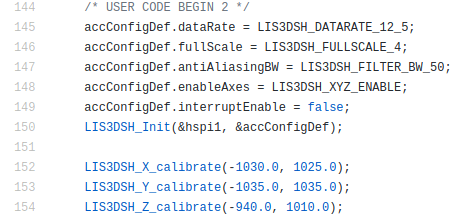
\includegraphics[width=\textwidth]{code_acc_config.png}
\caption{Code pour configurer l'accéléromètre}
\label{fig:accconfig}
\end{figure}

Les fonctions \texttt{calibrate} permettent de calibrer l'accéléromètre, c'est-à-dire faire en sorte que les valeurs minimales et maximales des accélérations soient le plus proches possible de -1000 et 1000. Les paramètres passés sont les accélérations minimales et maximales mesurées avant la calibration.

L'extrait de code en figure \ref{fig:accwhile} est celui qui récupère les valeurs de l'accéléromètre toutes les secondes, normalise les valeurs pour avoir l'échelle attendue par l'arbitre et enfin transmet les valeurs normalisées (\texttt{accMove}) au DevKit407. Ce code fait appel à la fonction \texttt{convertAccData} pour normaliser les données dont le code source est présenté en figure \ref{fig:accconvert}.

\begin{figure}[h]
\centering
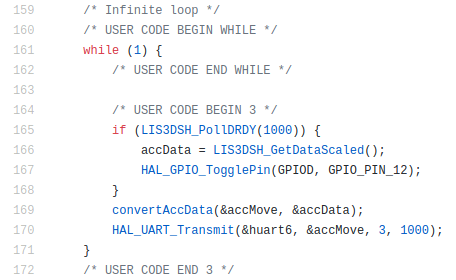
\includegraphics[width=\textwidth]{code_acc_while.png}
\caption{Code pour récupérer les accélérations et les transmettre}
\label{fig:accwhile}
\end{figure}

\begin{figure}[h]
\centering
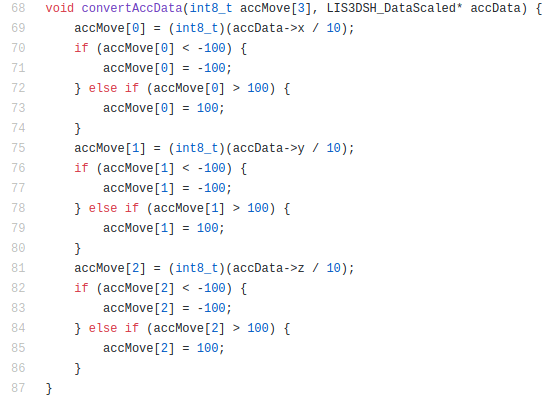
\includegraphics[width=\textwidth]{code_acc_convert.png}
\caption{Code pour normaliser les accélérations}
\label{fig:accconvert}
\end{figure}

\subsection{Communication entre les deux cartes}

La communication entre les deux cartes se fait via \texttt{UART}.

Les pins \texttt{UART6} de la carte \texttt{acc} sont connectées aux pins \texttt{UART5} de la carte \texttt{web}. \\

Les données transitant au sein de cette connection sont les données provenant de l'accéléromètre (en soi nous avons uniquement besoin d'envoyer des données de \texttt{acc} vers \texttt{web}, ainsi connecter toutes les pins UART n'est pas nécessaire).

Ces messages ont une taille de 3 bytes et contiennent:

\begin{itemize}
    \item L'accélération sur \texttt{x} encodée en \texttt{int8} sur 1 byte
    \item L'accélération sur \texttt{y} encodée en \texttt{int8} sur 1 byte
    \item L'accélération sur \texttt{z} encodée en \texttt{int8} sur 1 byte
\end{itemize}

\subsection{Intégration de la carte XBee}

La communication avec la carte \texttt{XBee} se fait également en UART, les pins \texttt{UART3} de la carte \texttt{web} sont connectées à la carte \texttt{XBee} (la carte \texttt{web} est également responsable de l'alimentation de la carte \texttt{XBee}).

Au niveau logiciel, la communication est gérée par la librairie définie dans le fichier \texttt{web/Src/bum\_player.c}.


\section{Conclusion}

Le projet permet de jouer au jeu BUMPERS en manipulant un microcontrôleur dans l'espace. Les accélérations du mouvement du joueur dictent la trajectoire de sa balle sur le plateau de jeu. Ceci nécessitait d'implémenter différents composants (accéléromètre, interface web, XBee) puis de les connecter entre eux. Implémenter chacun des composants ne représentait pas de grande difficulté. En revanche, faire en sorte qu'ils puissent se connecter et intéragir entre eux de manière cohérente fut un défi plus important.
Finalement, nous réussissons à présenter un projet quasiment terminé, mais nous avons recontré quelques difficultés, les principales étant :
\begin{itemize}
    \item Un flux de travail inhabituel, provoquant de ce fait quelques ralentissements. Par exemple, pour une expérience de développement optimale, deux ordinateurs portables étaient nécessaires dont un avec un port Ethernet.
    \item Un déverminage pas toujours évident. Bien sûr nous avons utilisé le dévermineur \texttt{gdb} mais nous avons aussi, par exemple, implémenté un script Python pour vérifier facilement que les bonnes données étaient transmises par la connexion UART.
\end{itemize}

Finalement, le projet était tout de même une bonne expérience qui nous a permis de nous familiariser une première fois avec le développement de logiciels embarqués pour des microcontrôleurs.

\end{document}

